\chapter{Практическая значимость задачи}

В настоящее время всё большее внимание уделяется принципиальной схеме самолета ``летающее крыло''. Данная схема применяется в том числе и для разработки беспилотных летательных аппаратов, предназначенных для разведки. В конструктировании таких самолетов особое внимание уделяется требованиям малозаметности и увеличения аэродинамического качества, и как слествие, возможности барражировать в течение длительного времени. 

Для удовлетворения данным требованиям конструкцию самолета создают максимально ``плоской'' -- так, в подобных конструкциях строительная высота фюзеляжа сравнима с высотой двигателя. Один из способов создания подобной конструкции -- использование изогнутого кессона. (Рис.\ref{fig:OriginalSectionWithEngine}). Примером такого самолета служит концепт американского беспилотного летательного аппарата RQ-180 (Рис.\ref{fig:rq180}). 

\begin{figure}[ht]
\centering
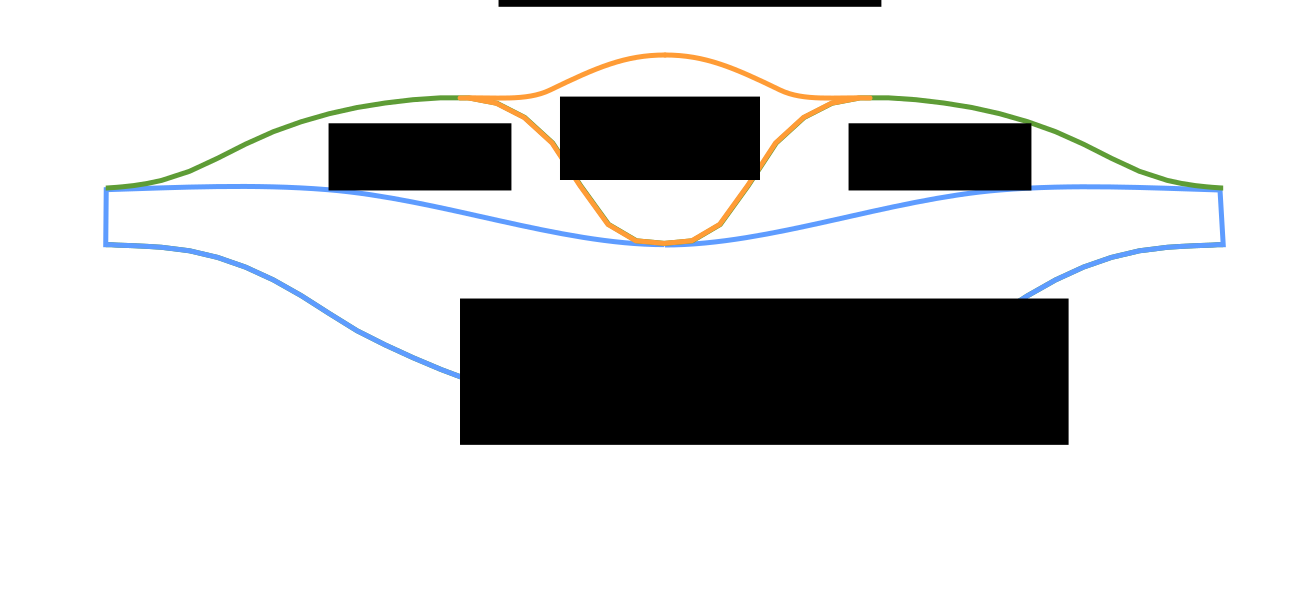
\includegraphics[width=0.7\textwidth]{OriginalSectionWithEngine}
\caption{Вид сечения центроплана в месте стыка передней кромки крыла и фюзеляжа с изображением двигателя}
\label{fig:OriginalSectionWithEngine}
\end{figure}

\begin{figure}[ht]
\centering
\includegraphics[width=0.6\textwidth]{rq180concept}
\caption{Концепт американского БПЛА RQ-180}
\label{fig:rq180}
\end{figure}

Так как вес конструкции является одним из важнейших критериев при выборе конструкции самолета, (что-то дописать), при проектировании самолета необходимо знать, какой вклад в вес конструкции совершает выбор такой формы кессона. С целью получения таких сведений в данной работе проводится анализ влияния различных форм кессона на вес самолета. 

Стоит заметить, что для того, чтобы в полной мере понимать целесообразность выбора той или иной формы центроплана, необходимо проводить комплексный анализ с учетом того, как меняются аэродинамических характеристик самолета при выборе той или иной формы кессона, и выбирать оптимальный вариант, исходя из критериев как прочности, так и аэродинамики. В данной работе проводится анализ лишь с точки зрения прочности конструкции, аэродинамические характеристики и нагрузки приняты постоянными. 

Полученные в работе данные возможно использовать при дальнейшем проектировании самолетов схемы ``летающее крыло''. 